\chapter{Obecné}


\section{Model architektury}

Ať už použijeme DDA s online nebo offline adaptivitou, implicitní nebo explicitní, je zde spousta společných rysů, a proto je na místě vytvořit obecný model architektury dynamického vyvažování obtížnosti. Ve všech případech se snažíme podchytit zjednodušený model hráče na základě jeho projevů ve hře, a poté tyto informace dodáme hře, která herní svět upraví k lepšímu zážitku hráče.

Jeden z možných modelů DDA znázorňuje obr. \ref{fig:ch2ddaarch}. V principu se zaznamenávají akce hráče a herní proměnné jako je např. počet životů hráče. Na základě těchto logů se vytváří model hráče, model jeho zkušeností, dovedností, preferencí a osobnosti. Model hráče v kombinaci s aktuálním stavem hry slouží k odhadu očekávaného zážitku hráče v dalším stavu hry. A nakonec model zážitku s model výkonu hráče slouží jako vstup adaptačnímu a generačnímu enginu, který posléze upraví herní komponenty jakými je např. umělá inteligence NPC.

\begin{figure}
  \centering
  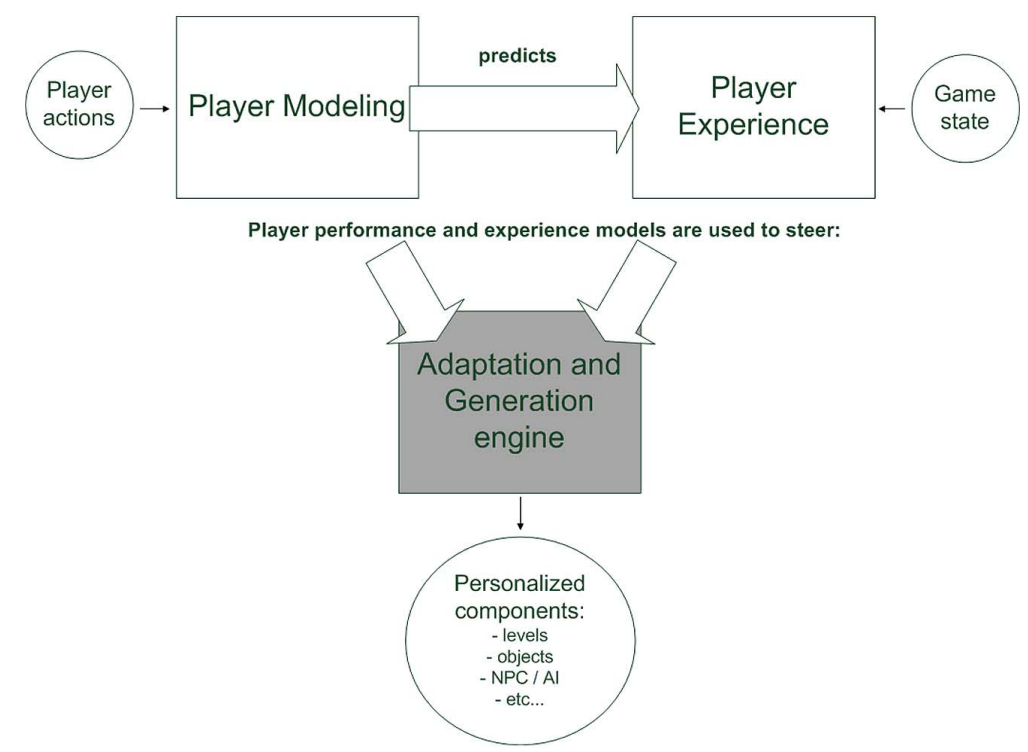
\includegraphics[width=0.75\textwidth]{ch2ddaarch}
	\caption{Přehled principů architektury adaptivních her. \cite{16Survey} }
	\label{fig:ch2ddaarch}
\end{figure}

V \cite{SwPatterns} se zabývali modelem DDA z pohledu návrhových vzorů objektového programování. Abstraktní model je znázorněn na obr. \ref{fig:ch2ddapatterns}. Senzory sbírají důležitá herní data, dle kterých se bude dále rozhodovat. Návrhový vzor Observer je připojen k Senzorům a v případě, že zaznamená zatelnou změnu v systému, vytvoří událost, trigger. Jednotlivé události jsou spojeny s akcemi a dohromady spolu tvoří pravidla uložená v databázi. V případě, že se spustí trigger spojený s akcí v některém z pravidel, rozhodne se v provedení této akce, což má na starost řadič, který má za úkol provést požadovanou změnu do stavu hry.

\begin{figure}
  \centering
  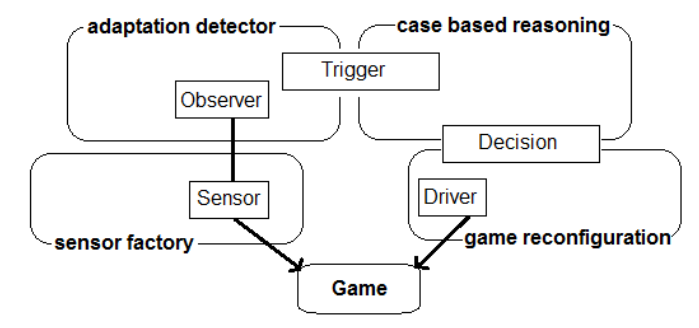
\includegraphics[width=0.75\textwidth]{ch2ddapatterns}
	\caption{Návrhové vzory DDA \cite{SwPatterns} }
	\label{fig:ch2ddapatterns}
\end{figure}

Dále se podíváme na jednotlivé návrhové vzory detailněji.

\subsection{Sensor factory}

Senzory jsou objekty, které pravidelně čtou herní data\footnote{Senzory nemusí zaznamenávat pouze herní data. Mohou zaznamenávat i prostředí uživatele např. pomocí Kinectu, nebo snímat aktuální tep hráče.} a upozorňují na změny zbytek DDA systému. Schéma návrhového vzoru znázorňuje obr. \ref{fig:ch2senzorfactory}. Senzor je abstraktní třídou, která zahrnuje periodické sbírání dat a upozorňující mechanismus. Konkrétní senzory z této třídy dědí a musí přepisovat abstraktní metodu refreshValue(), která zaznamenává konkrétní proměnnou systému. Třída SenzorFactory je zodpovědná za vytváření jednotlivých senzorů a je implementací návrhového vzoru factory. Továrna na senzory vyžaduje název senzoru a objekt, který má monitorovat. Vytvořené senzory si ukládá do registru. V případě, že uživatel zažádá o senzor, který už někdo vytvořil, dostane referenci na tento senzor. V opačném případě zkontroluje v ResourceManageru, jestli vytvořením nového senzoru se poruší některá z omezení zdrojů a pokud ne, senzor vytvoří.

\begin{figure}
  \centering
  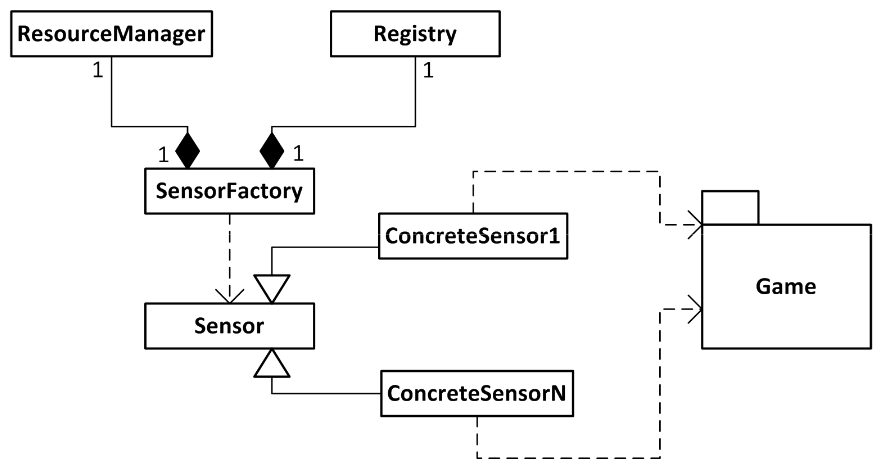
\includegraphics[width=0.5\textwidth]{ch2senzorfactory}
	\caption{Návrhový vzor sensor factory. \cite{SwPatterns} }
	\label{fig:ch2senzorfactory}
\end{figure}

\subsection{Adaptation detector}

Hrubá data získaná senzory se musí dále zpracovat. Tyto data získává AdaptationDetector pomocí observeru z návrhového vzoru senzor-observer. Na tomto místě se rozhoduje, jestli senzory již zaznamenaly dostatečnou změnu systému. Nedostatečnou změnou může být vystřelení jednoho náboje z plně nabitého revolveru. Naopak vystřílení půlky zásobníku může být významné. O významnost změny se stará TreshholdAnalyzer s Tresholdem. Treshold uchovává parametr hranice a její typ. (menší rovno, větší apod.) V případě dosažení prahu TresholdAnalyzer dá vědět AdaptationDetectoru, který vytvoří trigger, spouštěč. Trigger s sebou může nést další dodatečné informace jako je např. množství přeživších nepřátel. Viz obr. \ref{fig:ch2adaptationdesing}.

\begin{figure}
  \centering
  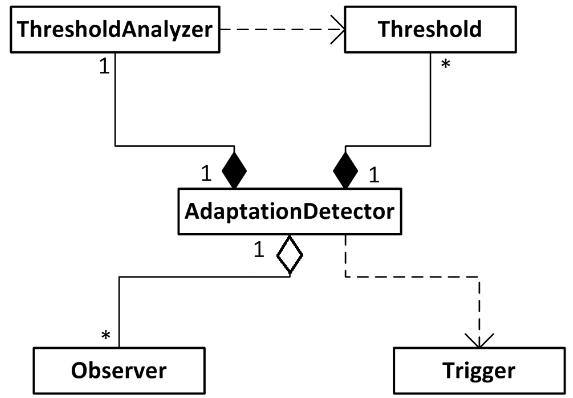
\includegraphics[width=0.5\textwidth]{ch2adaptationdesing}
	\caption{Návrhový vzor sensor factory. \cite{SwPatterns} }
	\label{fig:ch2adaptationdesing}
\end{figure}

\subsection{Case based reasoning}

Trigger spustí rozhodování na základě případů. Tento návrhový vzor(obr. \ref{fig:ch2casebase}) se použije, jestliže je možné vyvažování obtížnosti definovat konečným množstvím případů. InferenceEngine obsahuje dvě datové struktury: TriggerPool a FixedRules. Fixed rules obsahují pravidla, která jsou úzce spojená s konkrétní hrou. Pravidlo je kombinací triggeru a akce/rozhodnutí. TriggerPool funguje jako fronta událostí. Do fronty se řadí spuštěné triggery a jsou obsluhovány od nejstaršího. InferenceEngine vždy odebere jeden trigger z poolu, najde ho v databázi FixedRules pravidel a s ním nalezne vhodné rozhodnutí, které se má dále provést.

\begin{figure}
  \centering
  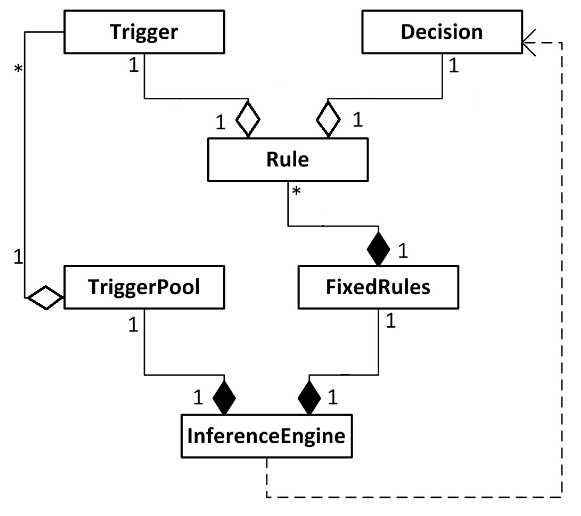
\includegraphics[width=0.5\textwidth]{ch2casebase}
	\caption{Návrhový vzor Case based reasoning. \cite{SwPatterns} }
	\label{fig:ch2casebase}
\end{figure}

\subsection{Game reconfiguration}

Posledním krokem je provedení požadované změny v herním světě. Návrhový vzor Game reconfiguration(obr. \ref{fig:ch2gamereco}) v sobě obsahuje jiný návrhový vzor, adapter. AdaptationDriver dostane ke zpracování rozhodnutí z InferenceEnginu. AdaptationDriver provede rozhodnutí za pomoci Driveru. Driver mění objekty, jež implementují rozhraní State, přes které zjišťuje aktuální stav objektu. S provedením jeho změny čeká dokud se nestane objekt neaktivním.

\begin{figure}
  \centering
  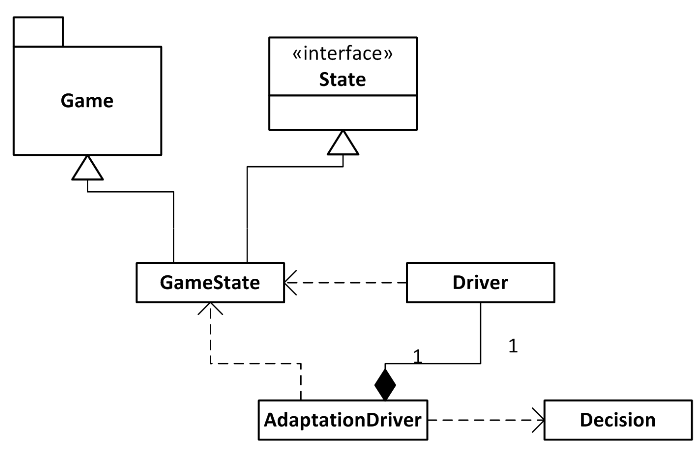
\includegraphics[width=0.5\textwidth]{ch2gamereco}
	\caption{Návrhový vzor Game reconfiguration. \cite{SwPatterns} }
	\label{fig:ch2gamereco}
\end{figure}

\section{Zábava}

Pojem zábava patří mezi velice subjektivní pojmy. Pro každého je zábavného něco jiného a svět her není výjimkou. Mezi hlavní zastupitele zkoumající tento pozitivní požitek patří Mihaly Csikszentmihalyi, který ideální stav maximální zábavy, maximálního ponoření do některé z činností nazval flow. Blíže tento stav bude popsán v následující podsekci.

Přestože se jedná o pojem subjektivní, pro použití DDA je nutné najít některé složky zábavy, které jsou změřitelné, kvantifikovatelné. Musíme být schopni zábavu měřit. Jestliže ji dokážeme změřit, můžeme to využít pro stavbu DDA algoritmů a i pro měření kvalit různých algoritmů mezi sebou. Možné metriky budou popsány dále.

\subsection{Flow}

Flow (tok) je stav mysli, kdy je osoba v průběhu provozování činnosti naprosto soustředěná, pociťuje nadšení, úspěch. „Flow je stav vědomí, kdy je člověk plně zaujatý svou činností. Nezabývá se jinými stimuly z okolí ani svými myšlenkami nebo pocity. Je naprosto soustředěný na prováděnou činnost. Dosahuje většinou, na své poměry, nadprůměrných výkonů, ale přitom mu to nepůsobí výraznou námahu. Je to harmonický zážitek, kdy tělo a mysl spolu bez námahy spolupracují. Tento stav je většinou spojen s pocity energie, radosti, harmonie a seberealizace.“ \cite{FlowCZ} S pojmem Flow prvně přišel zástupce pozitivní psychologie Mihaly Csikszentmihalyi ve své práci Flow: The psychology of optimal experience, česky vydané pod názvem O štěstí a smyslu života.

Požadovaný stav lze charakterizovat z pohledu dovedností člověka a náročnosti prováděné činnosti. Dosáhneme ho, jestliže provádíme úkol náročností odpovídající našim schopnostem. Viz obr. \ref{fig:ch2flow}. 

Jestliže se člověk seznamuje s novou činností, začíná v levém dolním rohu flow grafu. V tu chvíli nemá žádné dovednosti a pravděpodobně se začíná učit provádět činnost od jednoduchých částí po složitější. V knize \cite{OptimalFun} uvádí Csikszentmihalyi jako příklad takové činnosti hraní tenisu a vysvětluje to na obr. \ref{fig:ch2flow}. Alex začíná hrát tenis, a tedy se nachází ve fázi označené $A_1$. Alex v této chvíli neumí vůbec hrát tenis a začíná s tréninkem trefování se do míčku. Není to příliš obtížné, ale Alex si to užívá, protože náročnost tohoto úkolu přesně odpovídá jeho schopnostem.

\begin{figure}
  \centering
  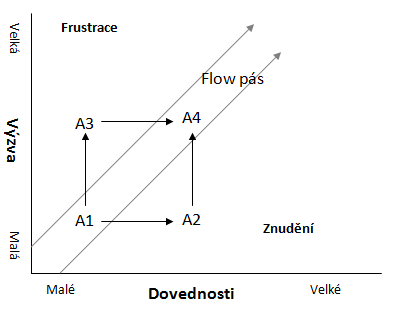
\includegraphics[width=0.5\textwidth]{ch2flow}
	\caption{Příklad pohybu jedince ve flow grafu. \cite{OptimalFun} }
	\label{fig:ch2flow}
\end{figure}

V této chvíli se Alex pohybuje v tzv flow pásu. Na stejném místě v diagramu nemůže zůstat Alex věčně. Jak danou činnost procvičuje, stává se v ní čím dál lepší, přestává ho to bavit, dostává se do nudy znázorněné v grafu $A_2$. V opačném případě se může stát, že potká zkušeného hráče. Hra proti němu je mnohem náročnějším úkolem a převyšuje Alexovy schopnosti. Alex se v takovém případě dostává do stavu úzkosti a stresu $A_3$.

V obou zmíněných příkladech se Alex nachází mimo flow pás a bude se snažit do něj opět dostat. V horším případě hru vzdá a další stav $A_4$ již v grafu nebude. V případě, že je ve stavu $A_2$, je dalším logickým krokem začít obtížnější úkol, vytyčit si nový cíl odpovídající jeho schopnostem. Ve stavu stresu $A_3$ má Alex jedinou možnost, zlepšit své dovednosti, aby se opět vrátil do flow pásu. Teoreticky může ubrat na výzvě, náročnosti úkolu, ale jak je jednou člověk vystaven takové výzvě, je pro něj těžké ji ignorovat a vzdát se jí. \cite{OptimalFun}

Dle Csikszentmihalyi se flow skládá z devíti elementů. \cite{FlowEng} Ne všechny jsou nutně potřebné k dosažení stavu flow.

\begin{enumerate}
	\item Jasné cíle
	\item Zpětná vazba
	\item Vyrovnanost náročnosti úkolů a schopností
	\item Splynutí činnosti a vědomí
	\item Koncentrace
	\item Žádné obavy z neúspěchu
	\item Pocit kontroly
	\item Změna vnímání času
	\item Vnitřní motivace
\end{enumerate}

Rozepisování jednotlivých bodů není záměrem této práce. Bližší informace lze nalézt např. na \cite{FlowEng}, \cite{FlowCZ}, nebo v originální knize \cite{OptimalFun}.

\subsubsection{Flow ve hrách}

Nás bude více zajímat napojení flow na vývoj počítačových her. Jenova Chen ve své diplomové práci Flow in Games\cite{thesisflow} vybral několik flow komponent, které označil za hlavní při návrhu hry. Dle Chena musí hra obsahovat následující tři elementy, aby hráč dosáhl stavu flow.

\begin{enumerate}
	\item Předpokladem je, že hra sama o sobě je pro hráče odměňující. Hráč sám o sobě chce hru hrát.
	\item Hra nabízí správnou náročnost úkolů vzhledem k hráčovým schopnostem, což mu umožňuje více se do hry ponořit.
	\item Hráč potřebuje cítit kontrolu nad prováděnou činností.
\end{enumerate}

Jsou-li splněny všechny tři body, hráč může ztratit pojem o čase a zcela se do hry ponořit.

Stavem flow ve hrách se dále zabýval Lennart Nacket, který ve svém článku\cite{FlowAll} shrnuje spojení flow s počítačovými hrami od různých autorů. Sweetserův a Wyethův herní flow osmi složkami vycházejícími z 9 složek flow od M. Csikszentmihalyi.

\begin{enumerate}
  \item Jasné cíle
	\item Zpětná vazba
	\item Výzva
	\item Hráčovi dovednosti
	\item Koncentrace
	\item Pocit kontroly
	\item Ponoření se do činnosti
	\item Sociální interakce
\end{enumerate}

\textbf{Jasné cíle} : 
Hráč by měl být vždy schopen kognitivně zpracovávat herní mise, úrovně, úkoly. Aktuální úkoly by měly být vždy jednoznačné a nematoucí. Hráč by měl být schopen vnímat svůj pokrok ve hře.

\textbf{Zpětná vazba} : 
Hra by měla vždy uživatele informovat o výsledku provedených akcí. Hráč by měl být seznámen, jak se blíží, či oddaluje od splnění cíle hry.

\textbf{Výzva} : 
U příliš jednoduchých her se nemohou uživatelé ponořit do hry. Hra musí být výzvou. Podstatné je rozlišovat náročnost ve formě špatně navrženého uživatelského rozhraní a ovládání a výzvu jako část herního designu. Špatné ovládání není nikdy žádoucí.

\textbf{Hráčovi dovednosti} : 
Hra by měla být navržena tak, aby hráči umožňovala efektivní získávání herních dovedností. Hra by měla brát v úvahu i možné dovednosti získané hráčem z jiných her.

\textbf{Koncentrace} : 
Hráč musí být do hry zcela ponořen, věnovat ji veškerou svojí pozornost.

\textbf{Pocit kontroly} : 
Hráč má mít pocit, že ovládá dění ve hře. Tento bod může být kritickým u návrhu DDA. Zjistí-li hráč, že jeho úspěch ve hře není zcela závislý na jeho výkonu, ztrácí pocit kontroly.

\textbf{Ponoření se do činnosti} : 
Podobné koncentraci. Hra má pohlcovat a udržovat hráče v maximální pozornosti, ale tak, aby mu to bylo stále příjemné.

\textbf{Sociální interakce} : 
Tento bod je přidán oproti prvotnímu flow. K dokonalému zážitku potřebuje člověk další lidské spoluhráče a protihráče.

\subsubsection{Zóna flow pro různé hráče}

Vraťme se znovu ke flow diagramu \ref{fig:ch2flow}. Dle příkladu s Alexem a jeho učením se tenisu by se mohlo zdát, že pro každého je ideální udržovat zcela vyrovnanou hodnotu schopností a náročnosti úkolů a udržovat uživatele v úzkém flow pásu, jak znázorňuje obr. \ref{fig:ch2flowzone1}.

\begin{figure}
  \centering
  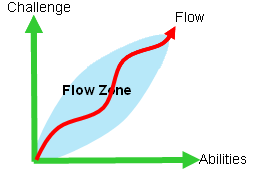
\includegraphics[width=0.5\textwidth]{ch2flowzone1}
	\caption{Obecně je vhodné hráče udržovat ve flow zóně. \cite{thesisflow} }
	\label{fig:ch2flowzone1}
\end{figure}	

Bohužel takový flow diagram nebere v úvahu individualitu hráče. Existují hráči, kteří mají rádi větší výzvy než jsou v tu chvíli schopni zvládnout, lze je nazvat hardcore hráči. Naopak existují příležitostní hráči, kteří netouží po velkých výzvách a nejraději se budou pohybovat lehce pod flow zónou. Těchto specifik si všímá např. práce \cite{RiskTakers}. Ideální průběh hry pro příležitostné/začínající hráče, běžné hráče a hardcore hráče znázorňuje graf na obr. \ref{fig:ch2flowzone2}. Mnohé práce tato specifika opomíjejí a často je jejich cílem upravit obtížnost hry, aby byl vyrovnaný počet hráčových výher a proher a už neberou v potaz, že někteří hráči přestanou hrát, když budou z poloviny pokusů prohrávat.

\begin{figure}
  \centering
  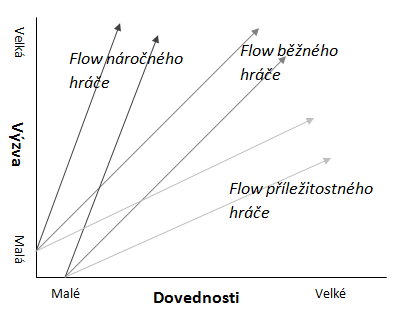
\includegraphics[width=0.5\textwidth]{ch2flowzone2}
	\caption{Flow zóna a specifika pro příležitostné a hardcore hráče. \cite{thesisflow} }
	\label{fig:ch2flowzone2}
\end{figure}	

\subsection{Metriky zábavnosti} \label{sec:defzab}

Hlavním cílem počítačových her je pobavení hráče. Může být tedy dobré umět zábavu přímo, či nepřímo změřit. Pro techniku DDA je existence takové metriky zcela zásadní. Bez ní by hra nevěděla, jakým způsobem se má přizpůsobovat hráči a neuměla by ohodnotit, jestli to dělá dobře. 

Metriky můžeme rozdělit do několika kategorií. Některé metriky jsou specifické pro konkrétní hru, jiné jsou obecně použitelné pro většinu existujících her. Dále jsou metriky, jež vycházejí pouze ze stavu hry, softwaru. Protikladem mohou být speciální metriky měřící hodnoty z vnějšího světa. Příkladem může sledování srdečního tepu \cite{7}. Dále lze využít webkameru, senzory na herních i neherních zařízení. Kromě tepu lze využívat např. pevnost stisku joysticku, měnící se odpor kůže, teplotu těla.\cite{16Survey} V této práci se pro naše účely zaměřím na metriky univerzálně použitelné a získané ze stavu hry.

Zábava ve hrách se často zjednodušuje do podoby náročnosti hry vzhledem k dovednostem hráče. Z tohoto důvodu velké množství přístupů pracuje s metrikami, které zábavu měří nepřímo, měří obtížnost hry. Často používanou metrikou je hodnota win-rate, poměr vítězstvích hráče ku jeho prohrám. Hodnota 0,5 značí polovinu výher a polovinu proher. Mnohé přístupy hodnotu 0,5 berou jako ideální. V tomto případě se hra snaží obtížnosti přiblížit co nejpřesněji dovednostem hráče. Jak bylo naznačeno v předchozí sekci, ne každý hráč ocení polovinu proher. Zde je prostor pro kombinaci statické a dynamické obtížnosti. Při statické obtížnosti si hráč vybere jednu z předem daných obtížností, např. začátečník, pokročilý, expert, kterým budou odpovídat hodnoty win-rate 25, 50, 75 %.

Další metriky využívají heuristiku, která numericky ohodnotí stav hry pro každého hráče a která nepřímo vyjadřuje pravděpodobnost výhry hráče. Samotná heuristika je herně specifická, ale prakticky u každé hry lze nějakou vymyslet, a proto jsou metriky, které ji využívají, obecně použitelné. Příkladem jednoduché heuristiky ve hře dáme bude počet zbývajících kamenů hráče. U hry Člověče, nezlob se může být jednoduchou heuristikou suma vzdáleností figur jednoho hráče od cíle.

V článku \cite{24DynLev} na základě zmíněné heuristiky přicházejí k třem metrikám. Počet změn ve vedení, napínavost během hry a konečný náskok. Hráč, který dle heuristiky má největší pravděpodobnost na výhru, je ve vedení. Jestliže se dostane do vedení jiný hráč, zaznamená se to. Metrika měří počet výměn hráčů ve vedení během hry od začátku do konce. Je zde předpoklad, že hra je více zábavná, jestliže se hráči častěji ve vedení střídají, a tedy není pořadí hráčů stejné na začátku, během a na konci hry. Napínavost je dána průměrným náskokem prvního hráče před druhým během hry. Konečný náskok je dán rozdílem heuristik prvního a druhého hráče na konci hry.

Všechny 4 zmíněné metriky (3 předchozí + win-rate) lze dobře využít v teorii her pro ohodnocení jednotlivých algoritmů a porovnání jich mezi sebou. Metriky doplníme o další tři nové. Počet výměn hráčů ve vedení nemusí být dostatečný. Mohlo by se stát, že každý z hráčů by byl během hry 2 krát ve vedení, ale jeden z nich by byl ve vedení 90\% času a zbylí hráči zbývajících 10\%. Metrika vedení bude udávat rozptyl časů ve vedení jednotlivých hráčů.

Jednou ze složek flow je kontrola. Hráč chce mít pocit vlády nad hrou. Jestliže budeme hru příliš často a hodně přizpůsobovat hráči, on/a si může všimnout, že nemá plnou kontrolu nad hrou, hra ho může přestat bavit. Proto by počet zásahů do hry měl být minimální. Spočítáme si pro každého hráče heuristiku vždy před adaptivním krokem $h_1$ a po něm $h_2$. Rozdíl $\Delta h = h_2 - h_1$ znázorňuje, jak moc jsme konkrétnímu hráči ublížili/pomohli k vítězství.  Můžeme vytvořit 2 nové metriky, kontrolu a spravedlnost. Kontrola bude dána průměrem z absolutních hodnot $\Delta h$ během hry na jednoho hráče. Trochu paradoxně, čím menší hodnota kontroly, tím lépe. Tím méně bylo zasaženo do hry. Pro spravedlnost je důležité během hry pomáhat/ubližovat všem přibližně stejně. Čím vyrovnanější $s(p) = \frac{1}{k}\sum_i^k \Delta h_i(p)$ na konci hry mezi jednotlivými hráči, tím lépe. Metrika spravedlnost je dáno rozptylem hodnot $s(p)$

\subsubsection{Algoritmus}

Pro lepší pochopení nastíněných metrik prohození prvních hráčů, napínavost, konečný náskok, vedení, kontrola, spravedlnost bude následovat pseudokód algoritmu(\ref{alg-metrik}) na výpočet zmíněných metrik. Mějme heuristickou funkci $H$, která má jediný argument, konkrétního hráče. Funkce vrací ohodnocení hráče v aktuálním stavu hry. Při inicializaci se zaznamenají heuristiky v čase 0. Nikdo z hráčů ještě nebyl ve vedení. Proměnné $pF_i$ a $pS_i$ zaznamenávají, který hráč byl v čase $i$ na první, respektive druhé pozici.

\begin{algorithm}
\caption{Výpočty metrik}
\label{alg-metrik}
\begin{algorithmic}[1]
\State $\forall p \in P : h_0(p) = H(p)$
\State $\forall p \in P : dobaVedeni(p) = 0$
\State $pF_0 = p_0$
\State $pF_t = 1$
\For{$i \gets 1, 2, \dots, k$}
   \State $\forall p \in P : h_i(p) = H(p)$
	 \State $pF_{i}  = \operatorname{arg\,max}_{p \in P} h_{i}(p)$
	 \State $pS_i = \operatorname{arg\,max}_{p \in P / pF_i} h_{k}(p)$
	 \If{$pF_i \neq pF_{i-1}$}
			\State $prohozeniVitezu = prohozeniVitezu + 1$
			\State $dobaVedeni(pF_{i-1}) = dobaVedeni(pF_{i-1}) + (i - pF_t)$
			\State $pF_t = i$
	 \EndIf
	 \State $DDA()$
	 \State $\forall p \in P : \Delta h_i(p) = H(p) - h_i(p)$
	 \State $ProvedTah()$
\EndFor
\State $\forall p \in P : s(p) = \frac{1}{k}\sum_i^k \Delta h_i(p)$
\State $\mu_s = \frac{1}{|P|}\sum_{p \in P} s(p)$
\State $\mu_v = \frac{1}{|P|}\sum_{p \in P} dobaVedeni(p)$
\State $napinavost = \frac{1}{k}\sum_i^k{h_i(pF_i) - h_i(pS_i)}$ 
\State $konecnyNaskok = h_k(pF_k) - h_k(pS_k)$
\State $vedeni = \sqrt{\sum_{p \in P} |\mu_v - dobaVedeni(p)|^2}$
\State $kontrola = \frac{1}{k |P|}\sum_i^k{\sum_{p \in P} |\Delta h_i(p)|}$
\State $spravedlnost = \sqrt{\sum_{p \in P} |\mu_s - s(p)|^2}$
\end{algorithmic}
\end{algorithm}

Následuje for smyčka přes časové okamžiky ve hře. U tahových her odpovídá časový okamžik stavu hry na začátku jednoho tahu. U realtime her je nutno čas rozdělit do pevných časových okamžiků. Ve smyčce se v každém čase zaznamená heuristika pro každého z hráčů a z ní určí hráči na prvních dvou pozicích. Jestliže se hráči na první pozici vystřídají, zvedne se hodnota heuristiky prohození prvních hráčů o jedničku a hráči, který byl do tohoto okamžiku ve vedení se připočte doba, po kterou byl naposledy ve vedení. Na řádku 14 se provede adaptivní krok hry. Zaznamená se rozdíl heuristik hráčů před a po adaptivním kroku. Na konci jednoho cyklu se provede další tah u tahové hry, případně se nechá hra běžet po nějakou dobu u realtime her.

Po skončení hry se mohou dopočíst heuristiky napínavost, konečný náskok, vedení, kontrola a spravedlnost dle popsaného významu dříve.


